    \textit{Author: Nursultan Shabykeev} \\
    \label{sec:rcf_sagemaker}
    \subsubsection{Motivation}
    Amazon SageMaker RCF is an algorithm for detecting anomalous data points within a data set. Generally, anomalies differ significantly from the majority of the data and usually manifest as unexpected breaks in periodicity or sudden high peaks in time series. After we plotted our data, we could easily see that it contained high spikes and we wanted to know whether the RCF model can identify these data points as anomalies and how well it is able to detect local anomalies. Besides, the fact that Random Cut Forest\footnote{Amazon RCF SageMaker is an implementation for batch data processing, not to be confused with Kinesis RCF which is designed for near real-time data processing.} is a built-in algorithm for Amazon SageMaker and can be easily deployed, additionally motivated us to try it out on our data set.
     
    \subsubsection{General idea}
    The main idea behind the algorithm is that it firstly takes a random sample of the training data and cuts them to the same number of points, i.e., the sample is partitioned into a number of equal-sized subsets. Then, each subset is assigned to an individual tree what leads to creation of a forest. The forest is later used to define whether a new data point is an anomaly. It is done by inserting a new point into the trees and determining how much that changes the complexity of the forest. If an average change of depth and width of trees highly increases, than a data point might be considered as anomalous. Generally, the algorithm assigns an anomaly score for each input data point. The higher a score, the more a data point differs from the majority of the data.\\
    
    Below, we describe creation and deployment of the RCF SageMaker model and as well as the final results. For the full and detailed explanation of RCF algorithm please see an official documentation \cite{awsRcfSagemaker}.
    
    \subsubsection{Training}
    The data consists of a number of requests (VPC Flowlogs from BMW) aggregated into one minute buckets. To train the model, we used the data over the course of one week that has "normal" behavior.  Then, we fed the whole data into the trained model for testing. We will present the test results later. Here, we describe important parts of the training process.\\
    
    \textbf{Hyperparameters}\\
    RCF model can be tuned with the following hyperparameters:
    \begin{itemize}
        \item \textit{num\textunderscore samples\textunderscore per\textunderscore tree} indicates the expected density of anomalies within the data. As a general rule, 1/\textit{num\textunderscore samples\textunderscore per\textunderscore tree} should approximate the estimated ratio of anomalies to normal points in the dataset. For example, if this value equals to 512, then we expect our data to contain anomalies 1/512 or approximately 0.2\% of the time.
   
        \item \textit{num\textunderscore trees} - the number of trees to create in the forest. Each tree learns a separate model from different samples of data. The full forest model uses the mean predicted anomaly score from each constituent tree \cite{awsRcfSagemaker}.
        \item \textit{feature\textunderscore dim} - the dimension of each data point.
    \end{itemize}
    Along with these RCF model hyperparameters, we provide additional parameters like the EC2 instance type on which training will run, the S3 bucket containing the data, and the AWS access role (see figure \ref{fig:rcf_model_training}). Note that,
    \begin{itemize}
        \item Recommended instance type: ml.m4, ml.c4, or ml.c5
        \item Current limitation: The RCF algorithm does not take advantage of GPU hardware \cite{awsRcfSagemaker}.
    \end{itemize}
    \begin{figure}[h]
        \centering
        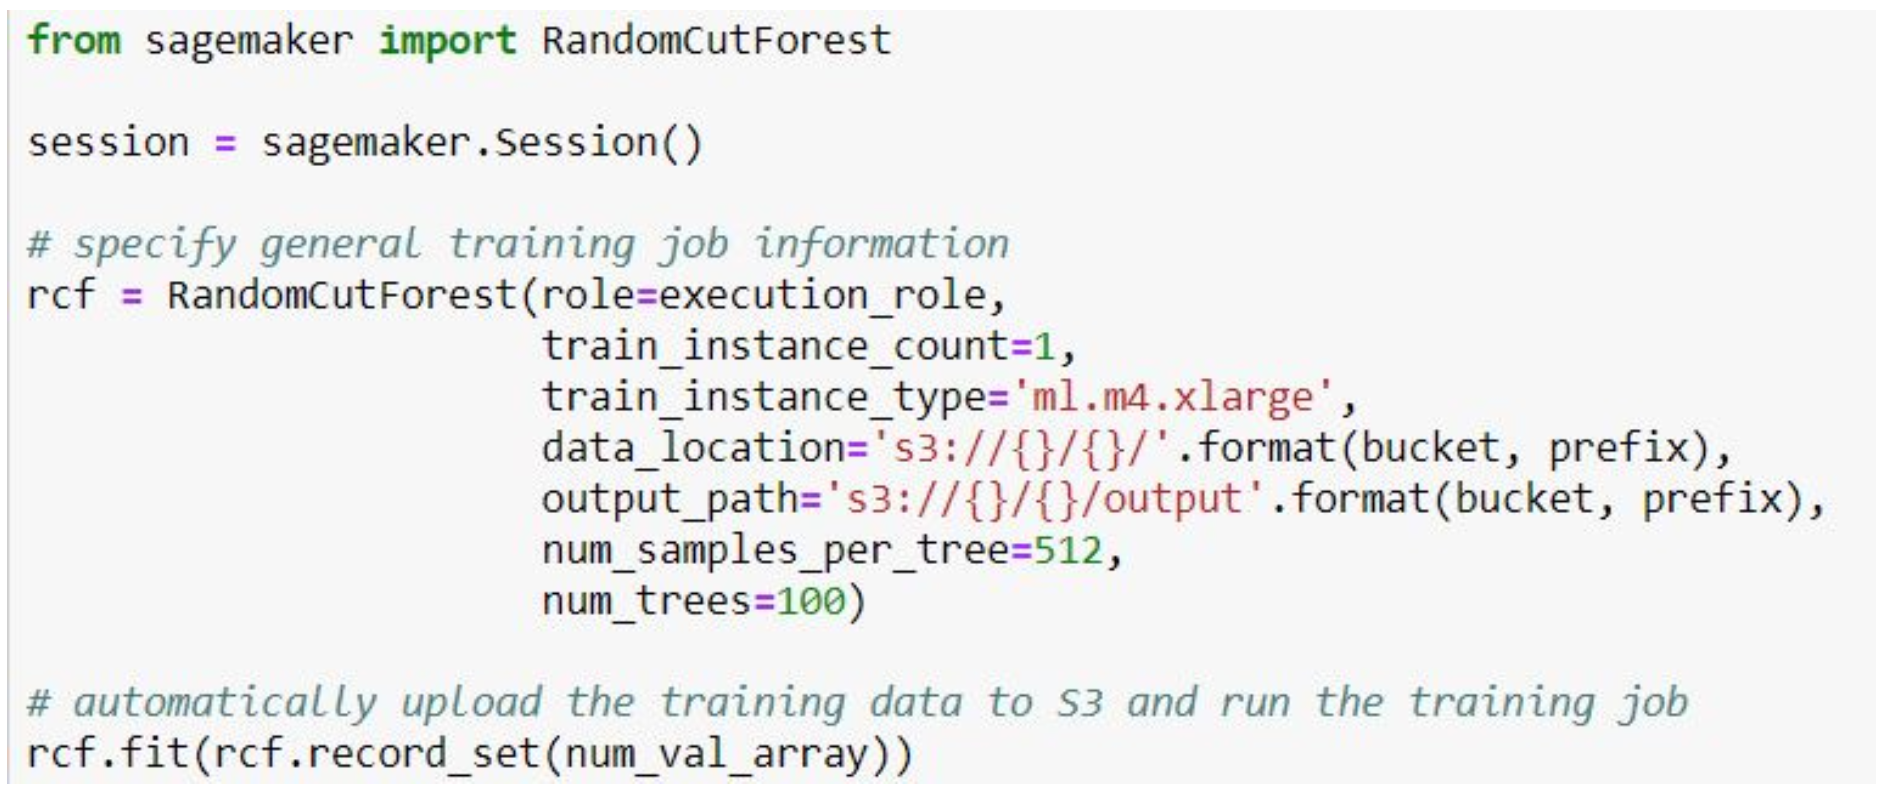
\includegraphics[width=0.85\textwidth]{images/rcf-model-training.png}
        \caption{RCF Model training}
        \label{fig:rcf_model_training}
    \end{figure}
    \FloatBarrier
    
    \subsubsection{Deployment}
    After the model is trained, we can to deploy it on an endpoint. We use \verb|SageMaker Python SDK deploy()| function from the job to create an inference endpoint. The function has two input parameters:  the instance type and an initial number of instances. Now using the deployed model, we can perform inference on the data. There are two ways to invoke the trained model:
    \begin{itemize}
        \item Right after training in the same notebook, calling a job’s \textit{predict(Test\textunderscore data)} function
        \item From elsewhere(e.g., inside a lambda function), using a function \textit{runtime.invoke\textunderscore endpoint\\(EndpointName, ContentType, Body)}
    \end{itemize}
    
    \subsubsection{Computing an anomaly threshold}
    RCF algorithm outputs an anomaly score for each input data point. 'Normal' data points are assigned low score values, whereas anomalous data points get high score values.
     Basically, a data point is considered to be anomalous if it is beyond a specific threshold. It is suggested in a RCF documentation \cite{awsRcfSagemaker}, to compute a value of an anomaly threshold as 3 standard deviations from the mean score. 
    Of course, the way to compute the threshold value is subject to change. Furthermore, another question is how to properly compute the threshold in terms of time, i.e., how long should a threshold stay valid. Depending on business requirements, one can calculate it either once for a whole period of data or for shorter periods of time, e.g., recompute threshold every day.\\
    For our data, we tried different ways of computing a threshold. Firstly, we computed it for the whole period of data, i.e., for almost one month. In this case, just evident peaks as on 2019-01-25 were beyond the threshold. Later, we decided to calculate the threshold per each day and these results are presented in figure \ref{fig:rcf_results}.
     \begin{figure}[h]
        \centering
        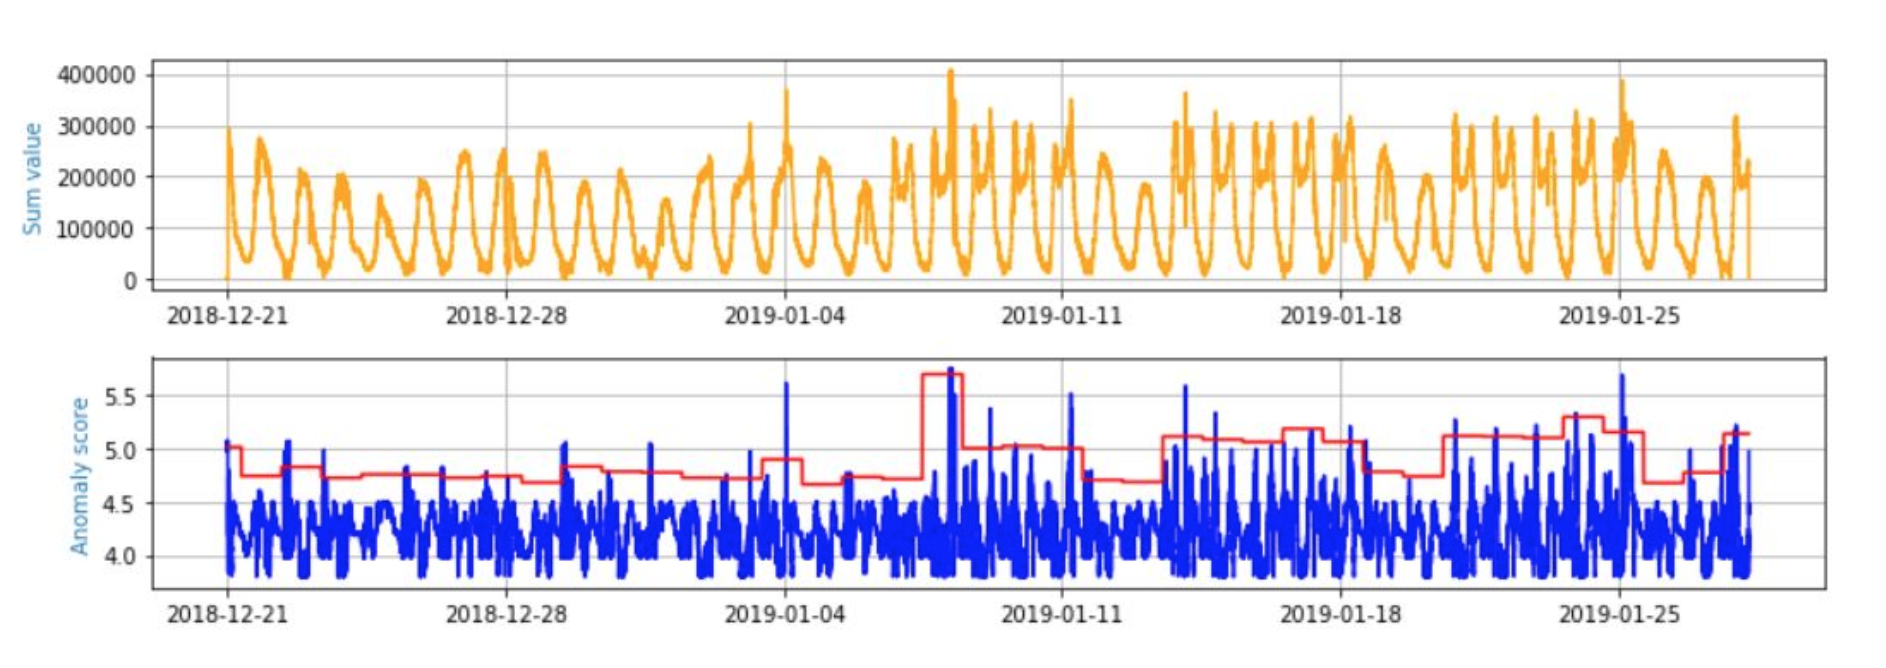
\includegraphics[width=1\textwidth]{images/rcf-results.png}
        \caption{Plotted data, anomaly scores, and anomaly threshold values}
        \label{fig:rcf_results}
    \end{figure}
    \FloatBarrier
    
    \subsubsection{Results}
    In figure \ref{fig:rcf_results}, the first plot represents the data, the second one demonstrates test results. The red plot depicts threshold values that we compute for each day. As we can see, not only high peaks are detected as anomalies, but also local downfalls (as on 2019-01-18) and congestion on bottoms (as on 2018-12-29) are anomaly candidates.
    
    In general, SageMaker RCF algorithm detects various types of anomalies on our data. Of course, some of found anomalies might not be anomalies at all in terms of application. One possible solution to this problem could be training the algorithm with more amount of data. In our case, we had the data just over the course of one month. Training a model with regularly repeating complex patterns might improve overall performance. Another technique is proper adjusting of a threshold, e.g., increasing it on holidays based on previous experience. 
   


